\section{Approach}
In this section we will describe our approach to the project, starting with the development methodology as described in Section 4.1. In Section 4.2 we present a broad overview of our system design. The programming languages and tools we will use for the project are specified in Sections 4.3 and 4.4 respectively. Finally, the API of FlightRadar24 will be introduced in Section 4.5.

\subsection{Development Methodology}
During the software development phase, the team will be applying agile development methods. In particular, the Scrum development framework will be used. Alternatives we have considered include the waterfall methodology and XP, extreme programming.

We have opted not to use the waterfall method due to its rigid and inflexible nature. For this project we foresee having to cope with design changes, which is difficult and time-consuming once implementation has started in the waterfall method. Throughout the project we will be implementing multiple mathematical models and designing a GUI that should be responsive and user-friendly in all situaions. In practice, the design of a GUI often has to go through multiple revisions to accomodate new requirements, incorporate new insights in the problem, etc. 

On the other hand, agile methods feature an iterative approach to software development, and are flexible enough to alter the design of a product throughout a project. As a result, using an agile method enables us to focus on the core of the product during initial stages, and add more functionality as the project progresses. It also allows us to keep a list of features that are not required for a functional product, but would increase its usefulness if implemented. These features can be reprioritized based on the client’s demands to ensure the final product contains the most requested and most valuable features that could be implemented in the limited timeframe.

Our choice for Scrum over XP as the preferred agile method is mainly based on experience of the team working with Scrum. On top of this, extreme programming is less suitable for small teams due to its strict requirements on code reviewing and testing, i.e., using pair programming. Due to the limited time available for this project, in some situations we prefer being able to work in parallel to ensure we cover more features. 
Additionally, in Scrum the work to be performed is planned in the sprint planning. We will work with one-week sprints. At the beginning of every week we will describe our goals for that week in a sprint plan. At the end of the week, all the items on the sprint plan need to be finished, fully tested and committed to the repository. A sprint reflection should also be made in which we discuss our progress during that sprint and possible improvements for the next sprint. Section 5 contains more detail on how we will ensure sufficient quality using our chosen methodology.

\subsection{System Overview}

\begin{figure}[ht]
    \centering
    \label{img:architecure}
    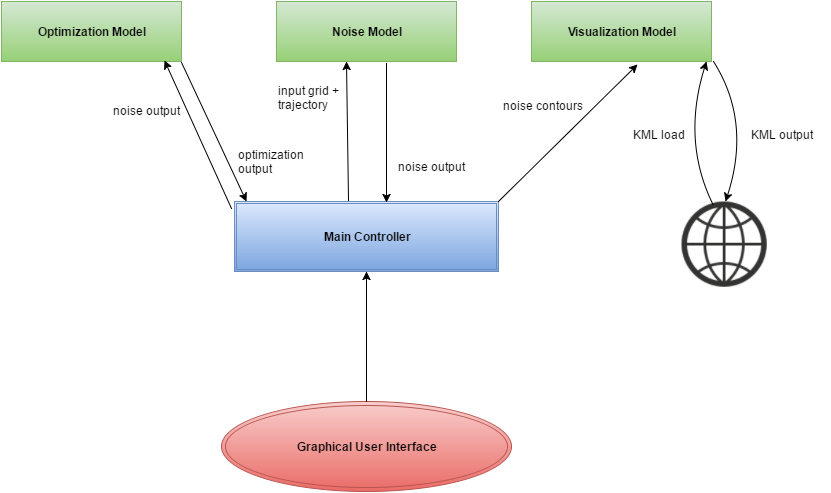
\includegraphics[width=0.75\textwidth]{images/EmergentArchitecture}
    \caption{A broad overview of the system architecture}
\end{figure}

As depicted in the diagram above, the models present the subsystems of our program. The Noise Model is responsible for the calculation of the noise values produced along a particular trajectory. Based on these noise values the Contour Model computes the noise contours that the user is interested in. Then
the Optimization Model updates a trajectory in an iterated manner based on the calculated noise contours. The KML Writer creates the KML files based on the (optimal) trajectory and its noise contours. These KML files will automatically be entered into Google Earth for visualization. Changes to the KML files will automatically be transferred to Google Earth by a 'KML load' script, which periodically loads the files into Google Earth.

The subsystems exchange their outputs with the main presenter which uses the output of one subsystem as input for the next one. This happens according to the following pipeline:

\begin{enumerate}
\item The main presenter enters the initial input file of the user into the Noise Model.
\item The main presenter passes on the output of the Noise Model to the Contour Model.
\item If the user selected the option to optimize, the main presenter relegates the output of the Contour Model to the Optimization Model. Otherwise, the output of the Contour Model is directly passed on to the KML Writer. When the output of the Contour Model is first handed over to the Optimization Model a loop is initiated: the current trajectory is updated by the Optimization Model and the workflow of the program starts all over again by entering the updated trajectory as input into the Noise Model. This optimization process is repeated until no further optimization is possible. 
\item The main presenter relegates the output of the Contour Model and the coordinates of the (optimal) trajectory to the KML Writer.
\end{enumerate}

Following this method the models are executed in a pipelined manner. But the subsystems will be designed in such a way that, given the right input files, the subsystems can also be run separately from each other and function as standalone applications.

\subsection{Programming Languages \& Libraries}

Because our program needs to solve optimization problems that require running computationally expensive calculations on a large amount of data points, code performance is an important factor. To this end, we hesitated between C++ and C\# and decided to compare them. 

C++ is known to be able to support high performance applications. However, we stumbled upon a few articles and blogs in which the performance of C++ was compared to C\#. All these articles noted that C++ itself does not have speed advantages. It is the fact that highly experienced programmers can express the strengths of the  language correctly which makes C++ code in some cases favorable over C\#. From these statements one can conclude that a performance-conscious C\# programmer can write programs with a performance similar to a well-written C++ program, however with the ease of being programmed in C\#. Since we both are not that experienced with C++, being able to write high quality C++ code and to actually achieve a higher performance would take practice and time to learn and thus would be very time consuming for us. This could even negatively affect the functionality of our program. Therefore, we believe that the use of C\# over C++ will increase our productivity. Even if a programmer succeeds to get a better performing implementation, the performance increase of C++ would probably not weigh up to the additional features that could have been added as a result of the time saved by programming in a more straightforward language. 

Besides that, C++ has cross platform capabilities whereas C\# depends upon the .NET framework which restricts its use to only the Windows platform. However, the benefit of having cross platform capabilities is not that important in our case since the client will use the software in combination with Matlab and Google Earth in a Windows environment. Therefore, we considered a few of the required components of our program with C++ and C\# in our minds. Our program needs to be able to generate XML files, PNG files and will make use of a library with a collection of common data structures. After a quick search on Internet we noticed that such libraries were more easy to find for C\#. Also, C\# is specifically designed to work with the .Net framework and is geared to the modern environment of Windows and user interface. Therefore C\# offers a lot more functionality and flexibility for GUI programming. With C++ you would have to hand code a lot of GUI functionality.

Mainly the first consideration regarding code performance and the GUI functionality that is built in C\# seemed to us as valid reasons for choosing C++ over C\#. To this end, we choose C\# as the main language for our code.

\paragraph{.NET Framework for GUI Development}
After we decided to choose C\# as the main language for our code, it was an obvious choice to develop our GUI with the .NET framework. The .NET Framework has become the mainstream environment for new Windows applications. It offers a lot of fancy options in case we decide to use innovative UI objects. Besides, the .NET framework contains a lot of predefined libraries for graph rendering and the creation of PNG's and color maps (which we are actually going to need for the visualization model). This helps to eliminate the amount of unnecessary codes and involves less coding for the developers. The framework also supports System.XML, which lets applications work with XML-defined data, including using XSLT and XPath. This comes in handy for us since we are going to use KML objects that are based on XML-defined data for the visualization model of our program.

But we still had to decide between using Windows Forms or WPF. The single most important difference between WinForms and WPF is the fact that while WinForms is simply a layer on top of the standard Windows controls (e.g. a TextBox), whereas WPF is built from scratch and doesn't rely on just the standard Windows controls. This might seem like a subtle difference, but it really isn't, which you will definitely notice if you are either creating a very complex or a relatively easy GUI. Since WinForms restricts users to a collection standard windows controls, a GUI that requires control elements that deviate from this is almost impossible to construct. By default WinForms for example does not support adding a background image to a ListView component. A programmer who really wants to seek the limits of what is graphically feasible will stumble upon a vast number of restrictions in WinForms. With WPF on the other hand control elements can be created by the designer in a container like fashion. In WPF for example a button with background image is created by adding a panel containing the image to the button. This is a great strength of WPF, however the current WPF form designer makes designing forms in WPF more tedious since you have to do significantly more work yourself. To give an example, the alignment of control elements requires more effort and is less obvious in WPF compared to WinForms. Since our GUI will mainly focus on requesting parameters that are required for performing the calculations, no complex control elements nor heavy graphics are necessary. Therefore, for our Windows application in which the standard Windows look and feel is expected WinForms will suffice and with the currently superior design environment will save us precious time.

\subsection{Tools usage}
In order to develop a product of this size, both development and process tools can help to keep an overview of the tasks at hand. In order to easily keep track of the increasing number of lines of code, a good IDE and some version control software can be very insightful. Similarly planning tools such as the agile-orientated JIRA can help to provide a clear overview of the current ToDo-list. In Section 4.5.1 we describe the development tools we will use in this project, whereas Section 4.5.2 will focus on the process tools.

\subsubsection{Functionality Tools}
\paragraph{INMTM v3.0} This noise calculation tool was provided by our client. It implements the FAA’s standard methodology for noise assessments and therefore the calculations in this tool are conform world standards. The client is really content with this tool since its execution time is less than one second. Therefore we decided to re-use the tool in our final program. In our minds we hold the option for further performance improvements in later stages of our project. The tool is written in Fortran so this means that, if we would like to improve the performance further, we would need to learn Fortran in a short period of time or we would need to rewrite the entire noise model from scratch. This is something we should take in consideration depending on the overall performance of our end product and the customer's needs.

\paragraph{Google Earth} Our client informed us that their preference goes out to visualization in Google Earth since this is commonly used in their research field. Besides, Google Earth provides a lot of options for satellite imagery of the entire earth in an interactive format. Compared to all its alternatives like Marble and Here Maps, Google Earth provides the most complete satellite imagery of the entire earth in 3D. One disadvantage of Google Earth is that the resolution of the image varies depending upon the location. This may make it more difficult for the user to view certain areas that are isolated or uninhabited. But since our visualization will mainly be located in the Netherlands and in populated areas surrounding airports, this should not be a problem for our program.

\subsubsection{Development tools}
As has been previously described in Section 4.4, we will develop the largest part of our code in C\#. For this part of the code, we will use Visual Studio. Visual Studio is both commonly used for C languages and is an IDE we have experience with. The alternative in the form of SharpDevelop has been considered, but since we have experience with Visual Studio, we believe this will allow for a smoother workflow and switching to the similar but slightly different SharpDevelop would hold no advantages. In contrast to an extensive IDE such as Eclipse, the alternative of Vim has also been considered. Vim is a command-line text editor that offers many development features for those that are used to its somewhat peculiar set of shortcuts. The downside is that for large projects it is quite difficult to keep a clear overview of all code. 

In addition to an IDE, we will also require version control to easily keep track of code changes. Version control systems manage changes in code and/or documents, and provide a central location to store the code and documents. We choose Git as our version control tool. Our project team has experience with both Git and SVN, and both version control systems are commonly used in academia and industry. As we are using an agile development method, a working version of the product, preferably with new features, should be presentable at the end of every sprint. To maintain a stable version of the product, branched development can be a huge benefit. This allows for a main branch that contains the proven to be stable version of the software, with new features being developed in separate branches. Because Git has built-in support for branch-based development, it is preferred over SVN which offers a very primitive branching system which involves manually creating the folders for branches and merging them afterwards.

Given that the core of our application is written in C\#, multiple testing frameworks are available. Out of the different options we decided to go with NUnit, since it is the most similar one to JUnit  which the team has the most experience with. Additionally, NUnit integrates seamlessly with Visual Studio and it fully supports test class inheritance. MsTest has slightly more features for test logging, but we still choose for NUnit due to it’s native support in Visual Studio and our previous positive experience with JUnit.

\subsubsection{Process tools}

In addition to the tools required for the development, we are also using a planning tool to keep track of our planning. JIRA is an online tool that allows for an overview of the current work, as well as some scrum-oriented features. One of these features is the scrum board which mimics the structure of ToDo, Work in Progress, Done that is often done with sticky notes on a white board. 

\subsection{API}

\paragraph{FlightRadar24 for real-time flight data}
For visualization of real flight routes we are going to use the API of FlightRadar24 to gather real-time air flight data. Its current version provides the broadest coverage of aggregated flight tracks and abstract information. The data is retrieved by a network of ADS-B receivers. FlightRadar24 does not provide a public API but they have a streaming endpoint for their data in JSON. We will be using a PHP API which is developed by a third party and provides all these data in JSON.

We considered the alternative API of FlightAware. They seem to have better routes/ flight plan data than FlightRadar24 but their feed is 5 minutes delayed. Because we want to visualize real flight routes (near) real-time, the delayed feed is no option for us. Another potential alternative is the OpenSky Network. This is a free open-source API that provides live visualization of air traffic and a real-time flight data feed. In contrast to FlightRadar24 it also offers access to historical raw data which would be very useful for testing our program. However, the location data feed is not that accurate and it contains no information on the flight status, such as the type of plane.
